

\tikzset{every picture/.style={line width=0.75pt}} %set default line width to 0.75pt        

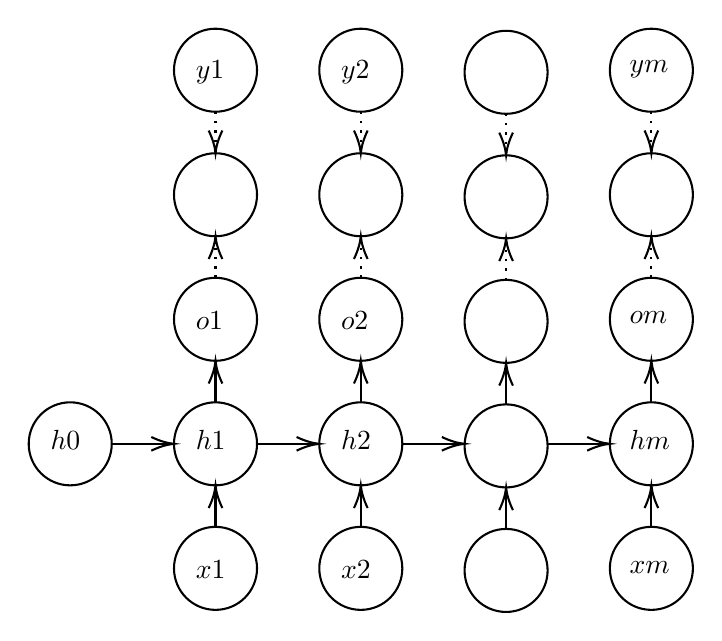
\begin{tikzpicture}[x=0.75pt,y=0.75pt,yscale=-1,xscale=1]
%uncomment if require: \path (0,323); %set diagram left start at 0, and has height of 323

%Shape: Circle [id:dp3629561388056113] 
\draw   (90,150) .. controls (90,138.95) and (98.95,130) .. (110,130) .. controls (121.05,130) and (130,138.95) .. (130,150) .. controls (130,161.05) and (121.05,170) .. (110,170) .. controls (98.95,170) and (90,161.05) .. (90,150) -- cycle ;
%Shape: Circle [id:dp44819185014685403] 
\draw   (160,150) .. controls (160,138.95) and (168.95,130) .. (180,130) .. controls (191.05,130) and (200,138.95) .. (200,150) .. controls (200,161.05) and (191.05,170) .. (180,170) .. controls (168.95,170) and (160,161.05) .. (160,150) -- cycle ;
%Shape: Circle [id:dp4778230592944719] 
\draw   (300,150) .. controls (300,138.95) and (308.95,130) .. (320,130) .. controls (331.05,130) and (340,138.95) .. (340,150) .. controls (340,161.05) and (331.05,170) .. (320,170) .. controls (308.95,170) and (300,161.05) .. (300,150) -- cycle ;
%Shape: Circle [id:dp4172940080920504] 
\draw   (90,210) .. controls (90,198.95) and (98.95,190) .. (110,190) .. controls (121.05,190) and (130,198.95) .. (130,210) .. controls (130,221.05) and (121.05,230) .. (110,230) .. controls (98.95,230) and (90,221.05) .. (90,210) -- cycle ;
%Shape: Circle [id:dp9221856908591408] 
\draw   (160,210) .. controls (160,198.95) and (168.95,190) .. (180,190) .. controls (191.05,190) and (200,198.95) .. (200,210) .. controls (200,221.05) and (191.05,230) .. (180,230) .. controls (168.95,230) and (160,221.05) .. (160,210) -- cycle ;
%Shape: Circle [id:dp5107698459287944] 
\draw   (300,210) .. controls (300,198.95) and (308.95,190) .. (320,190) .. controls (331.05,190) and (340,198.95) .. (340,210) .. controls (340,221.05) and (331.05,230) .. (320,230) .. controls (308.95,230) and (300,221.05) .. (300,210) -- cycle ;
%Shape: Circle [id:dp9971969777197274] 
\draw   (90,270) .. controls (90,258.95) and (98.95,250) .. (110,250) .. controls (121.05,250) and (130,258.95) .. (130,270) .. controls (130,281.05) and (121.05,290) .. (110,290) .. controls (98.95,290) and (90,281.05) .. (90,270) -- cycle ;
%Shape: Circle [id:dp6035985742831749] 
\draw   (160,270) .. controls (160,258.95) and (168.95,250) .. (180,250) .. controls (191.05,250) and (200,258.95) .. (200,270) .. controls (200,281.05) and (191.05,290) .. (180,290) .. controls (168.95,290) and (160,281.05) .. (160,270) -- cycle ;
%Shape: Circle [id:dp20977751188714566] 
\draw   (300,270) .. controls (300,258.95) and (308.95,250) .. (320,250) .. controls (331.05,250) and (340,258.95) .. (340,270) .. controls (340,281.05) and (331.05,290) .. (320,290) .. controls (308.95,290) and (300,281.05) .. (300,270) -- cycle ;
%Shape: Circle [id:dp23609841012892163] 
\draw   (90,30) .. controls (90,18.95) and (98.95,10) .. (110,10) .. controls (121.05,10) and (130,18.95) .. (130,30) .. controls (130,41.05) and (121.05,50) .. (110,50) .. controls (98.95,50) and (90,41.05) .. (90,30) -- cycle ;
%Shape: Circle [id:dp5318607092141312] 
\draw   (160,30) .. controls (160,18.95) and (168.95,10) .. (180,10) .. controls (191.05,10) and (200,18.95) .. (200,30) .. controls (200,41.05) and (191.05,50) .. (180,50) .. controls (168.95,50) and (160,41.05) .. (160,30) -- cycle ;
%Shape: Circle [id:dp7028223312018156] 
\draw   (300,30) .. controls (300,18.95) and (308.95,10) .. (320,10) .. controls (331.05,10) and (340,18.95) .. (340,30) .. controls (340,41.05) and (331.05,50) .. (320,50) .. controls (308.95,50) and (300,41.05) .. (300,30) -- cycle ;
%Shape: Circle [id:dp42488579033193763] 
\draw   (90,90) .. controls (90,78.95) and (98.95,70) .. (110,70) .. controls (121.05,70) and (130,78.95) .. (130,90) .. controls (130,101.05) and (121.05,110) .. (110,110) .. controls (98.95,110) and (90,101.05) .. (90,90) -- cycle ;
%Shape: Circle [id:dp1754771414071341] 
\draw   (160,90) .. controls (160,78.95) and (168.95,70) .. (180,70) .. controls (191.05,70) and (200,78.95) .. (200,90) .. controls (200,101.05) and (191.05,110) .. (180,110) .. controls (168.95,110) and (160,101.05) .. (160,90) -- cycle ;
%Shape: Circle [id:dp8997928679194878] 
\draw   (300,90) .. controls (300,78.95) and (308.95,70) .. (320,70) .. controls (331.05,70) and (340,78.95) .. (340,90) .. controls (340,101.05) and (331.05,110) .. (320,110) .. controls (308.95,110) and (300,101.05) .. (300,90) -- cycle ;
%Straight Lines [id:da8537414640186041] 
\draw    (110,250) -- (110,232) ;
\draw [shift={(110,230)}, rotate = 450] [color={rgb, 255:red, 0; green, 0; blue, 0 }  ][line width=0.75]    (10.93,-3.29) .. controls (6.95,-1.4) and (3.31,-0.3) .. (0,0) .. controls (3.31,0.3) and (6.95,1.4) .. (10.93,3.29)   ;
%Straight Lines [id:da8728240272525218] 
\draw    (180,250) -- (180,232) ;
\draw [shift={(180,230)}, rotate = 450] [color={rgb, 255:red, 0; green, 0; blue, 0 }  ][line width=0.75]    (10.93,-3.29) .. controls (6.95,-1.4) and (3.31,-0.3) .. (0,0) .. controls (3.31,0.3) and (6.95,1.4) .. (10.93,3.29)   ;
%Straight Lines [id:da3702106006623287] 
\draw    (320,250) -- (320,232) ;
\draw [shift={(320,230)}, rotate = 450] [color={rgb, 255:red, 0; green, 0; blue, 0 }  ][line width=0.75]    (10.93,-3.29) .. controls (6.95,-1.4) and (3.31,-0.3) .. (0,0) .. controls (3.31,0.3) and (6.95,1.4) .. (10.93,3.29)   ;
%Straight Lines [id:da8147113194897551] 
\draw    (110,190) -- (110,172) ;
\draw [shift={(110,170)}, rotate = 450] [color={rgb, 255:red, 0; green, 0; blue, 0 }  ][line width=0.75]    (10.93,-3.29) .. controls (6.95,-1.4) and (3.31,-0.3) .. (0,0) .. controls (3.31,0.3) and (6.95,1.4) .. (10.93,3.29)   ;
%Straight Lines [id:da9940060129323278] 
\draw    (180,190) -- (180,172) ;
\draw [shift={(180,170)}, rotate = 450] [color={rgb, 255:red, 0; green, 0; blue, 0 }  ][line width=0.75]    (10.93,-3.29) .. controls (6.95,-1.4) and (3.31,-0.3) .. (0,0) .. controls (3.31,0.3) and (6.95,1.4) .. (10.93,3.29)   ;
%Straight Lines [id:da21234167773916912] 
\draw    (320,190) -- (320,172) ;
\draw [shift={(320,170)}, rotate = 450] [color={rgb, 255:red, 0; green, 0; blue, 0 }  ][line width=0.75]    (10.93,-3.29) .. controls (6.95,-1.4) and (3.31,-0.3) .. (0,0) .. controls (3.31,0.3) and (6.95,1.4) .. (10.93,3.29)   ;
%Straight Lines [id:da51949842029655] 
\draw  [dash pattern={on 0.84pt off 2.51pt}]  (110,130) -- (110,112) ;
\draw [shift={(110,110)}, rotate = 450] [color={rgb, 255:red, 0; green, 0; blue, 0 }  ][line width=0.75]    (10.93,-3.29) .. controls (6.95,-1.4) and (3.31,-0.3) .. (0,0) .. controls (3.31,0.3) and (6.95,1.4) .. (10.93,3.29)   ;
%Straight Lines [id:da6212732550300433] 
\draw  [dash pattern={on 0.84pt off 2.51pt}]  (180,130) -- (180,112) ;
\draw [shift={(180,110)}, rotate = 450] [color={rgb, 255:red, 0; green, 0; blue, 0 }  ][line width=0.75]    (10.93,-3.29) .. controls (6.95,-1.4) and (3.31,-0.3) .. (0,0) .. controls (3.31,0.3) and (6.95,1.4) .. (10.93,3.29)   ;
%Straight Lines [id:da5634341890894232] 
\draw  [dash pattern={on 0.84pt off 2.51pt}]  (320,130) -- (320,112) ;
\draw [shift={(320,110)}, rotate = 450] [color={rgb, 255:red, 0; green, 0; blue, 0 }  ][line width=0.75]    (10.93,-3.29) .. controls (6.95,-1.4) and (3.31,-0.3) .. (0,0) .. controls (3.31,0.3) and (6.95,1.4) .. (10.93,3.29)   ;
%Straight Lines [id:da7517812400746318] 
\draw  [dash pattern={on 0.84pt off 2.51pt}]  (110,50) -- (110,68) ;
\draw [shift={(110,70)}, rotate = 270] [color={rgb, 255:red, 0; green, 0; blue, 0 }  ][line width=0.75]    (10.93,-3.29) .. controls (6.95,-1.4) and (3.31,-0.3) .. (0,0) .. controls (3.31,0.3) and (6.95,1.4) .. (10.93,3.29)   ;
%Straight Lines [id:da23656264229534862] 
\draw  [dash pattern={on 0.84pt off 2.51pt}]  (180,50) -- (180,68) ;
\draw [shift={(180,70)}, rotate = 270] [color={rgb, 255:red, 0; green, 0; blue, 0 }  ][line width=0.75]    (10.93,-3.29) .. controls (6.95,-1.4) and (3.31,-0.3) .. (0,0) .. controls (3.31,0.3) and (6.95,1.4) .. (10.93,3.29)   ;
%Straight Lines [id:da2050152758610957] 
\draw  [dash pattern={on 0.84pt off 2.51pt}]  (320,50) -- (320,68) ;
\draw [shift={(320,70)}, rotate = 270] [color={rgb, 255:red, 0; green, 0; blue, 0 }  ][line width=0.75]    (10.93,-3.29) .. controls (6.95,-1.4) and (3.31,-0.3) .. (0,0) .. controls (3.31,0.3) and (6.95,1.4) .. (10.93,3.29)   ;
%Straight Lines [id:da15141952791941238] 
\draw    (130,210) -- (158,210) ;
\draw [shift={(160,210)}, rotate = 180] [color={rgb, 255:red, 0; green, 0; blue, 0 }  ][line width=0.75]    (10.93,-3.29) .. controls (6.95,-1.4) and (3.31,-0.3) .. (0,0) .. controls (3.31,0.3) and (6.95,1.4) .. (10.93,3.29)   ;
%Straight Lines [id:da8773526556001805] 
\draw    (270,210) -- (298,210) ;
\draw [shift={(300,210)}, rotate = 180] [color={rgb, 255:red, 0; green, 0; blue, 0 }  ][line width=0.75]    (10.93,-3.29) .. controls (6.95,-1.4) and (3.31,-0.3) .. (0,0) .. controls (3.31,0.3) and (6.95,1.4) .. (10.93,3.29)   ;
%Shape: Circle [id:dp46244560624869613] 
\draw   (20,210) .. controls (20,198.95) and (28.95,190) .. (40,190) .. controls (51.05,190) and (60,198.95) .. (60,210) .. controls (60,221.05) and (51.05,230) .. (40,230) .. controls (28.95,230) and (20,221.05) .. (20,210) -- cycle ;
%Straight Lines [id:da797513658170024] 
\draw    (60,210) -- (88,210) ;
\draw [shift={(90,210)}, rotate = 180] [color={rgb, 255:red, 0; green, 0; blue, 0 }  ][line width=0.75]    (10.93,-3.29) .. controls (6.95,-1.4) and (3.31,-0.3) .. (0,0) .. controls (3.31,0.3) and (6.95,1.4) .. (10.93,3.29)   ;
%Straight Lines [id:da47947220492213916] 
\draw    (200,210) -- (228,210) ;
\draw [shift={(230,210)}, rotate = 180] [color={rgb, 255:red, 0; green, 0; blue, 0 }  ][line width=0.75]    (10.93,-3.29) .. controls (6.95,-1.4) and (3.31,-0.3) .. (0,0) .. controls (3.31,0.3) and (6.95,1.4) .. (10.93,3.29)   ;
%Shape: Circle [id:dp11600406730745116] 
\draw   (230,151) .. controls (230,139.95) and (238.95,131) .. (250,131) .. controls (261.05,131) and (270,139.95) .. (270,151) .. controls (270,162.05) and (261.05,171) .. (250,171) .. controls (238.95,171) and (230,162.05) .. (230,151) -- cycle ;
%Shape: Circle [id:dp9283593321630528] 
\draw   (230,211) .. controls (230,199.95) and (238.95,191) .. (250,191) .. controls (261.05,191) and (270,199.95) .. (270,211) .. controls (270,222.05) and (261.05,231) .. (250,231) .. controls (238.95,231) and (230,222.05) .. (230,211) -- cycle ;
%Shape: Circle [id:dp20021078146964966] 
\draw   (230,271) .. controls (230,259.95) and (238.95,251) .. (250,251) .. controls (261.05,251) and (270,259.95) .. (270,271) .. controls (270,282.05) and (261.05,291) .. (250,291) .. controls (238.95,291) and (230,282.05) .. (230,271) -- cycle ;
%Shape: Circle [id:dp7478548742855309] 
\draw   (230,31) .. controls (230,19.95) and (238.95,11) .. (250,11) .. controls (261.05,11) and (270,19.95) .. (270,31) .. controls (270,42.05) and (261.05,51) .. (250,51) .. controls (238.95,51) and (230,42.05) .. (230,31) -- cycle ;
%Shape: Circle [id:dp576916828524171] 
\draw   (230,91) .. controls (230,79.95) and (238.95,71) .. (250,71) .. controls (261.05,71) and (270,79.95) .. (270,91) .. controls (270,102.05) and (261.05,111) .. (250,111) .. controls (238.95,111) and (230,102.05) .. (230,91) -- cycle ;
%Straight Lines [id:da3104260432223389] 
\draw    (250,251) -- (250,233) ;
\draw [shift={(250,231)}, rotate = 450] [color={rgb, 255:red, 0; green, 0; blue, 0 }  ][line width=0.75]    (10.93,-3.29) .. controls (6.95,-1.4) and (3.31,-0.3) .. (0,0) .. controls (3.31,0.3) and (6.95,1.4) .. (10.93,3.29)   ;
%Straight Lines [id:da6924180302501548] 
\draw    (250,191) -- (250,173) ;
\draw [shift={(250,171)}, rotate = 450] [color={rgb, 255:red, 0; green, 0; blue, 0 }  ][line width=0.75]    (10.93,-3.29) .. controls (6.95,-1.4) and (3.31,-0.3) .. (0,0) .. controls (3.31,0.3) and (6.95,1.4) .. (10.93,3.29)   ;
%Straight Lines [id:da20416614901863794] 
\draw  [dash pattern={on 0.84pt off 2.51pt}]  (250,131) -- (250,113) ;
\draw [shift={(250,111)}, rotate = 450] [color={rgb, 255:red, 0; green, 0; blue, 0 }  ][line width=0.75]    (10.93,-3.29) .. controls (6.95,-1.4) and (3.31,-0.3) .. (0,0) .. controls (3.31,0.3) and (6.95,1.4) .. (10.93,3.29)   ;
%Straight Lines [id:da5869670003982028] 
\draw  [dash pattern={on 0.84pt off 2.51pt}]  (250,51) -- (250,69) ;
\draw [shift={(250,71)}, rotate = 270] [color={rgb, 255:red, 0; green, 0; blue, 0 }  ][line width=0.75]    (10.93,-3.29) .. controls (6.95,-1.4) and (3.31,-0.3) .. (0,0) .. controls (3.31,0.3) and (6.95,1.4) .. (10.93,3.29)   ;

% Text Node
\draw (99,265) node [anchor=north west][inner sep=0.75pt]    {$\Elem{x}{1}$};
% Text Node
\draw (169,265) node [anchor=north west][inner sep=0.75pt]    {$\Elem{x}{2}$};
% Text Node
\draw (240,269) node [anchor=north west][inner sep=0.75pt]    {$\dotsc $};
% Text Node
\draw (308,265) node [anchor=north west][inner sep=0.75pt]    {$\Elem{x}{m}$};

% Text Node
\draw (29,202) node [anchor=north west][inner sep=0.75pt]    {$\Elem{h}{0}$};
% Text Node
\draw (99,202) node [anchor=north west][inner sep=0.75pt]    {$\Elem{h}{1}$};
% Text Node
\draw (169,202) node [anchor=north west][inner sep=0.75pt]    {$\Elem{h}{2}$};
% Text Node
\draw (240,209) node [anchor=north west][inner sep=0.75pt]    {$\dotsc $};
% Text Node
\draw (308,202) node [anchor=north west][inner sep=0.75pt]    {$\Elem{h}{m}$};


% Text Node
\draw (99,145) node [anchor=north west][inner sep=0.75pt]    {$\Elem{o}{1}$};
% Text Node
\draw (169,145) node [anchor=north west][inner sep=0.75pt]    {$\Elem{o}{2}$};
% Text Node
\draw (240,149) node [anchor=north west][inner sep=0.75pt]    {$\dotsc $};
% Text Node
\draw (308,145) node [anchor=north west][inner sep=0.75pt]    {$\Elem{o}{m}$};

% Text Node
\draw (103,83) node [anchor=north west][inner sep=0.75pt]    {$\Loss$};
% Text Node
\draw (173,83) node [anchor=north west][inner sep=0.75pt]    {$\Loss$};
% Text Node
\draw (243,83) node [anchor=north west][inner sep=0.75pt]    {$\Loss$};
% Text Node
\draw (313,83) node [anchor=north west][inner sep=0.75pt]    {$\Loss$};

% Text Node
\draw (99,24) node [anchor=north west][inner sep=0.75pt]    {$\Elem{y}{1}$};
% Text Node
\draw (169,24) node [anchor=north west][inner sep=0.75pt]    {$\Elem{y}{2}$};
% Text Node
\draw (240,29) node [anchor=north west][inner sep=0.75pt]    {$\dotsc $};
% Text Node
\draw (308,24) node [anchor=north west][inner sep=0.75pt]    {$\Elem{y}{m}$};


\end{tikzpicture}